\begin{frame}[label=title]
    \centering
    \begin{figure}[H]
        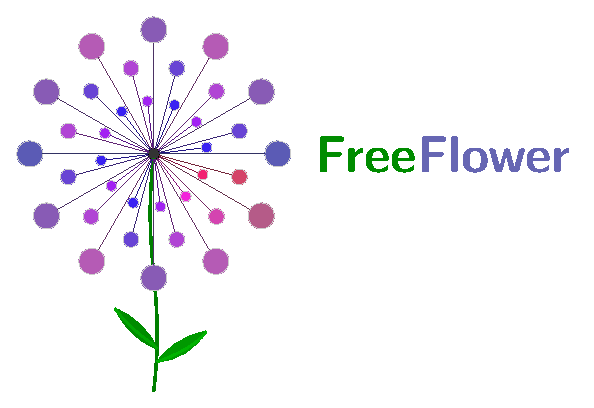
\includegraphics[keepaspectratio, width=0.7\paperwidth, height=\paperheight]{Logos/FreeFlower.pdf}
    \end{figure}
    Informatik: Data Science und Sicherheit\\
    \emoji{clamp}\textbf{Kompression}: Arithmetische Kompression
\end{frame}

\begin{frame}
\begin{columns}
\begin{column}{.5\textwidth}
Huffman-Kodierung
\begin{itemize}[<+->]
\item Optimale Kodierung von Zeichen.
\item Wenn die Häufigkeiten der Zeichen bei 1/2, 1/4, 1/8, etc. liegen, gibt es keine bessere Kodierung
\item Wenn eine Häufigkeit aber z.B. bei 30\% liegt, sind 2 Bits (optimal für 25\%) verschwenderisch!
\end{itemize}
\end{column}
\begin{column}{.5\textwidth}
\begin{figure}[H]
\centering
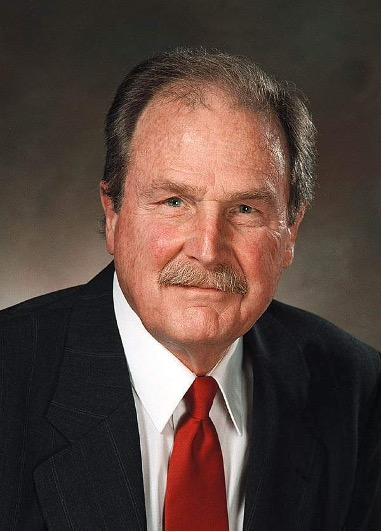
\includegraphics[width=\columnwidth]{Grundlagen_Info/04_Kompression/Figures/david_huffman}
\caption{David A. Huffman}
\label{fig:davidhuffman}
\end{figure}
\end{column}
\end{columns}
\end{frame}

\begin{frame}
\begin{columns}
\begin{column}{.5\textwidth}
Jorma Rissanen
\begin{itemize}[<+->]
\item Ganze Texte anstatt einzelne Buchstaben kodieren!
\item Idee: Jedem Text wird eine Zahl zwischen 0 und 1 zugeordnet
\item Je länger der Text, desto mehr Nachkommastellen
\item Ist unter gewissen Umständen kürzer als Huffman
\end{itemize}
\end{column}
\begin{column}{.5\textwidth}
\begin{figure}[H]
\centering
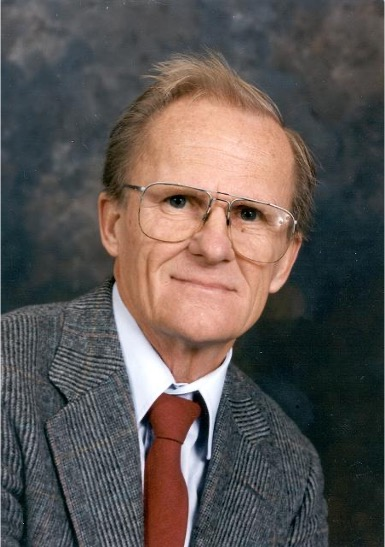
\includegraphics[width=\columnwidth]{Grundlagen_Info/04_Kompression/Figures/jorma_rissanen}
\caption{Jorma Rissanen}
\label{fig:jorma}
\end{figure}
\end{column}
\end{columns}
\end{frame}

\begin{frame}[fragile]{Arithmetische Kompression}
\vspace{-.5cm}
\begin{columns}
\begin{column}{.5\textwidth}
\begin{table}[H]
\centering
\footnotesize
\begin{tabular}{c||c|c|c|c}
\textbf{Buchstabe} & A & B & C & D \\\midrule
\textbf{Häufigkeit (\%)} & 50 & 20 & 20 & 10 \\
\end{tabular}
\end{table}
\end{column}
\begin{column}{.5\textwidth}
Wie wird der Text \texttt{ADBA} kodiert?
\end{column}
\end{columns}
\vspace{-.5cm}
\newcommand{\arithmeticTikz}[7]{
% 1st argument: height
% 2nd argument: increments
% 3rd argument: xPosL
% 4th argument: letters
% 5th argument: position of shift letter
% 6th argument: start of interval
% 7th argument: end of interval
	% Draw the initial line
    \draw (0,#1) -- (10,#1);   
	
%	\pgfmathsetmacro{\endCoord}{#2[3]+#3[3]}
	
	% draw 
    \foreach \i in {1,...,4}{
	    \pgfmathsetmacro{\inc}{#2[\i-1]} % increment for current interval
	    \pgfmathsetmacro{\xStart}{#3[\i-1]} % percentage at interval start
	    \pgfmathsetmacro{\xEnd}{\xStart+\inc} % percentage at interval end
	    \pgfmathsetmacro{\l}{#4[\i-1]} % label at middle of interval	    

		% draw vertical marks on main initial line
        \draw (\xStart*10,#1+0.2) to (\xStart*10,#1-0.2);
        \draw (\xEnd*10,#1+0.2) to (\xEnd*10,#1-0.2);
        
        % annotate interval start & end
        \node (\l-Perc) at (\xStart*10,#1-0.4) {\fpeval{round(((1-\xStart)*#6+#7*\xStart),4)}};
        \node (\l-PercEnd) at (\xEnd*10,#1-0.4) {\fpeval{round(((1-\xEnd)*#6+#7*\xEnd),4)}};
        % Increase y position for the next line 
        
        % draw brace and probabilities above line
        \ifnum\i=#5
        	\draw[decoration={brace,raise=5pt},decorate,red]
            	    (\xStart*10,#1+.2) -- node[above=6pt,text width=2cm, align=center] {\textcolor{red}{\texttt{\l{}}\\ (\pgfmathparse{int(round(\inc*100))}\pgfmathresult \%)}} (\xEnd*10,#1+.2);
        \else
	        \draw[decoration={brace,raise=5pt},decorate]
                    	    (\xStart*10,#1+.2) -- node[above=6pt,text width=2cm, align=center] {\texttt{\l{}}\\ (\pgfmathparse{int(round(\inc*100))}\pgfmathresult \%)} (\xEnd*10,#1+.2);
        \fi
    }
}
\begin{figure}[H]
\centering
\begin{tikzpicture}[yscale=.55]
\small\arithmeticTikz{4}{{0.5,0.2,0.2,0.1}}{{0,0.5,0.7,0.9}}{{"A","B","C","D"}}{1}{0}{1}
\only<2->{\arithmeticTikz{1}{{0.5,0.2,0.2,0.1}}{{0.5,0.6,0.2,0.7}{0,0.5,0.7,0.9}}{{"AA","AB","AC","AD"}}{4}{0}{.5}
% highlight transition area (L0 to L1)
\draw[-, red, dashed](0*10,4)--(0*10,1);
\draw[-, red, dashed](.5*10,4)--(1*10,1);
}
\only<3->{\arithmeticTikz{-2}{{0.5,0.2,0.2,0.1}}{{0.5,0.6,0.2,0.7}{0,0.5,0.7,0.9}}{{"ADA","ADB","ADC","ADD"}}{2}{.45}{.5}
% highlight transition area (L1 to L2)
\draw[-, red, dashed](.9*10,1)--(0*10,-2);
\draw[-, red, dashed](1*10,1)--(1*10,-2);
}
\only<4->{\arithmeticTikz{-5}{{0.5,0.2,0.2,0.1}}{{0.5,0.6,0.2,0.7}{0,0.5,0.7,0.9}}{{"ADBA","ADBB","ADBC","ADBD"}}{1}{.475}{.485}
% highlight transition area (L2 to L3)
\draw[-, red, dashed](.9*10,1)--(0*10,-2);
\draw[-, red, dashed](1*10,1)--(1*10,-2);
% highlight transition area (L3 to L4)
\draw[-, red, dashed](.5*10,-2)--(0*10,-5);
\draw[-, red, dashed](.7*10,-2)--(1*10,-5);}

\end{tikzpicture}
%\caption{Arithmetische Kodierung des Worts \texttt{ADBA}}
%\label{fig:arithm-kod}
\end{figure}
\end{frame}
\begin{frame}{Nachteil von arithmetischer Kodierung}
Komprimieren und Dekomprimieren ist mit Huffman effizienter $\rightarrow$ Abwägen (\textit{trade-off}) zwischen Speicherplatz und Rechenaufwand 
\end{frame}
\begin{frame}[label=auftrag]{Auftrag}
	\begin{itemize}
		\item \aufgabebox{Aufgaben 1.10, 1.11}
		\item \challengebox{Aufgabe 1.12}
	\end{itemize}
\end{frame}